\documentclass[11pt]{article}
\usepackage[margin=1in]{geometry}
\usepackage{amsmath,amssymb}
\usepackage{graphicx}
\usepackage{enumitem}
\usepackage{xcolor}
\usepackage{parskip}

\title{Rebuttal\\\large \emph{No-Regret Learning in Stackelberg Security
Games with an Unknown, Bounded Set of Attacker Types}}
\author{}
\date{}

\begin{document}
\maketitle
\vspace{-2em}

\noindent We thank both reviewers for their careful reading. Below we address every
question. Section / equation references are to the submitted report;
the labelling issue raised by Reviewer~2 is addressed in R2.Q1/Q3.

\section*{Reviewer 1}

\paragraph{R1.Q1 (Second \textsc{Grow-Catalogue} variant).}
We had originally planned a second variant with lazy recomputation of
$\mathcal E(C_t;\varepsilon)$, but dropped it during implementation.
The mentions in Section~7.2 and the corresponding row in Table~1 are
leftovers from earlier drafts and will be removed.

\paragraph{R1.Q2 (Validity of the Step~7 bound in our experimental regime).}
That's correct. After applying $\log(1+x)\le x$ in Eq.~(17) the
correction term we discarded is $K_{\max}\,n^{3}/2^{\,n-1}$, which we
treated as $O(1)$ on the basis $n^{3}/2^{n}=O(1)$. This is true
asymptotically in $n$, but is not a numerical bound at small $n$. The bound should therefore be read as
\[
\log N_{\max} \;=\; O\!\left(n^{2}+K_{\max}\log n\right)
\]
holding with an \emph{explicit} multiplicative constant that
absorbs the small-$n$ correction. The proof of Theorem~6 uses only the
asymptotic form of Eq.~(17), so the regret bound is unaffected.

\paragraph{R1.Q3 (Match with Balcan et al.\ Theorem~5.1).}
Our bound
$\widetilde O\!\left(\sqrt{T\cdot K_{\max}\cdot(n^{2}+K_{\max}\log n)}\right)$
does \emph{not} reduce literally to Balcan et al.\ Theorem~5.1 with
$k\!\leftarrow\!K_{\max}$. The intended statement is weaker: like
their bound, ours is sub-linear in $T$ under an appropriate scaling
regime on $K_{\max}$. We make that regime precise in Corollary~7,
namely $K_{\max}=o\!\left(\min(T/n^{2},\sqrt{T/\log n})\right)$. 

\paragraph{R1.Q4 (Experiments at larger $n$).}
We re-ran the per-round-regret experiment at $n=5$, $K_{\max}=4$,
$T=6000$ (20 seeds, non-uniform epochs $\ell=(300,800,1700,3200)$),
using a sampled $\varepsilon$-net for $\mathcal E$ since exact
enumeration is too expensive (R1.Q5). The proof of Theorem~6 only
requires a finite $\varepsilon$-cover, so the regret bound still
holds with a negligible additive $\varepsilon T$ term.
Figure~\ref{fig:n5_nonuniform} shows the same qualitative picture
as $n=3$: spike at each type-reveal, $O(t^{-1/2})$ decay within each
epoch, rolling mean returning to $\approx 0$ in the long final epoch.

\begin{figure}[h]
\centering
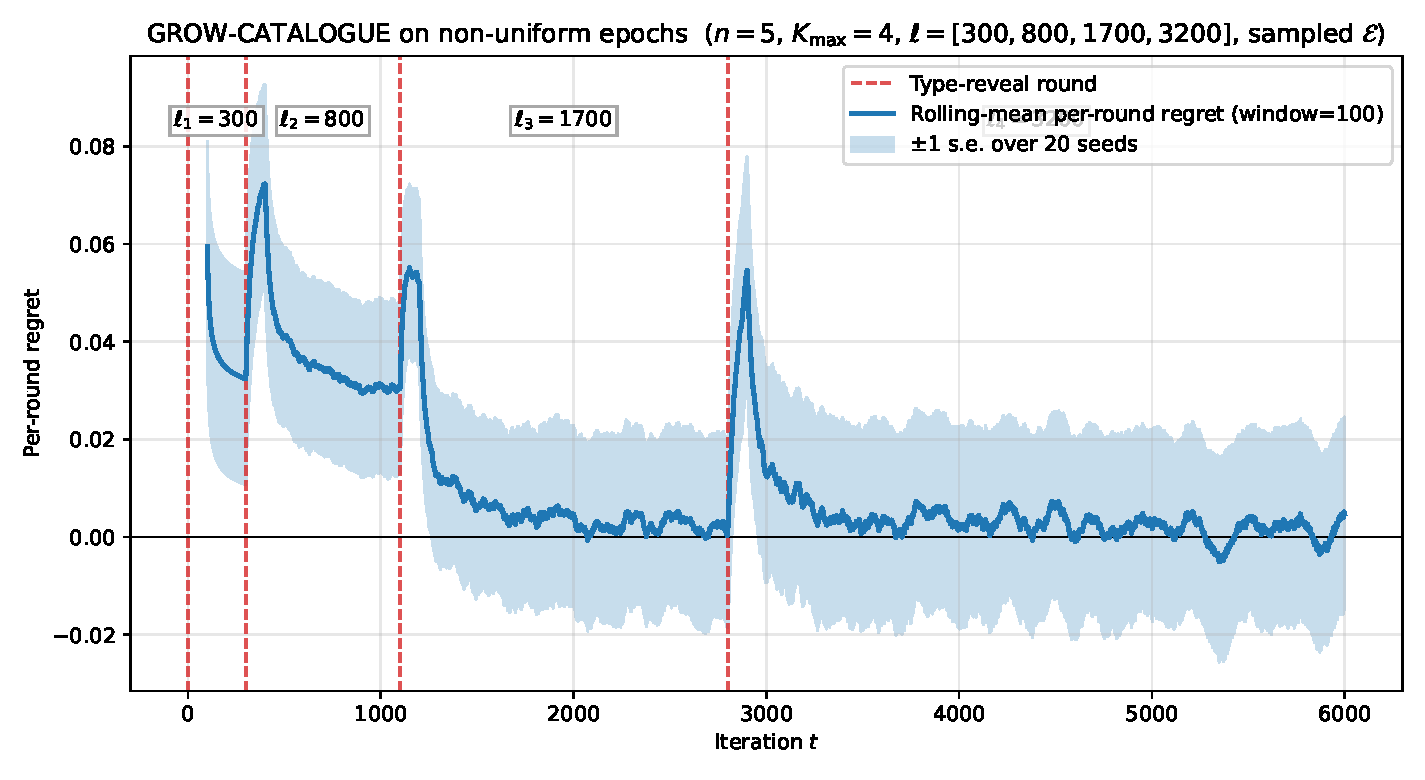
\includegraphics[width=0.92\linewidth]{figures/per_round_regret_n5_nonuniform.pdf}
\caption{Rebuttal experiment: $n=5$, $K_{\max}=4$, $T=6000$, non-uniform
epochs $\ell=(300,800,1700,3200)$, sampled $\varepsilon$-cover ($M=2000$),
mean $\pm 1$ s.e.\ over 20 seeds.}
\label{fig:n5_nonuniform}
\end{figure}

\paragraph{R1.Q5 (Runtime cost of $\mathcal E(C;\varepsilon)$ per discovery round).}
With $|C|=K$ and $n$ targets, exact enumeration intersects every
$(n-1)$-subset of the $n+K\binom{n}{2}$ defining hyperplanes, giving
$T_{\text{exact}}(n,K)=O(K^{n-1}\,\mathrm{poly}(n))$ for fixed $n$.
The sampling method of R1.Q4 costs only $O(MKn)$ per discovery, so it
removes the $K^{n-1}$ blow-up. Measured on a laptop ($n=5$, mean over
20 seeds):
\begin{itemize}[leftmargin=2em,itemsep=1pt,topsep=1pt]
\item Exact enumeration:
$K{=}1\!:\,80$\,ms ($|\mathcal E|{=}148$),
$K{=}2\!:\,6.13$\,s ($1578$),
$K{=}3\!:\,77.7$\,s ($6057$),
$K{=}4\!:\,349$\,s ($13794$).
\item Sampled $\varepsilon$-net:
$K{=}1\!:\,4.8$\,ms ($|\mathcal E|{\approx}4$),
$K{=}2\!:\,9.1$\,ms ($10$),
$K{=}3\!:\,13.4$\,ms ($21$),
$K{=}4\!:\,17.6$\,ms ($38$).
\end{itemize}
This cost is paid at most $K_{\max}$ times per run, so amortised over
$T$ it is negligible.

\paragraph{R1.Q6 (Definition of $q_t$).}
Inside epoch $i$, let $\mathcal E_i = \mathcal E(C_i;\varepsilon)$ with
$N_i=|\mathcal E_i|$, and $L^{(t)}(p)=\sum_{s=1}^{t-1}\ell^{(s)}(p)$
the cumulative loss. The Polynomial-Weights distribution is
\begin{equation}
q_t(p) \;=\;
\frac{\exp\!\left(-\eta_t\, L^{(t)}(p)\right)}
     {\sum_{p'\in\mathcal E_i}\exp\!\left(-\eta_t\, L^{(t)}(p')\right)},
\qquad
\eta_t \;=\; \sqrt{\log N_i / t},
\label{eq:qt}
\end{equation}
the anytime Hedge schedule of~\cite{CesaBianchi2007,CL06}. In
practice the algorithm keeps the cumulative losses
$\{L^{(t)}(p)\}_{p\in\mathcal E_i}$ in log space, recomputes
$\eta_t$ each round, normalises via a numerically-stable softmax to
obtain $q_t$, and then draws $p_t$ as a single categorical sample
over $\mathcal E_i$. 

\paragraph{R1.Q7 (Bandit / imperfect-information extension).}
Extending to bandit feedback (only the attacked target observed,
not the type) looks difficult: without type feedback the discovery
step is no longer well-defined, so sub-linear regret in full
generality seems implausible. A natural direction is to restrict to
special classes of attacker types (e.g.\ well-separated
best-response cells or a margin / identifiability condition) under
which sub-linear regret may still be achievable.

\paragraph{R1.Q8 (Full publication and main technical gaps).}
Yes, we are interested in extending this to a full publication. The
main directions we would pursue are (i) replacing the exact
$\mathcal E(C;\varepsilon)$ enumeration with a principled approximate
algorithm that is provably sub-linear in regret while keeping a
decent runtime at larger $n$, and (ii) tightening the dependence on
$n$ and $K_{\max}$ in the regret bound.

\section*{Reviewer 2}

\paragraph{R2.Q1 / R2.Q3 (Numbering of Theorems / Lemmas / Propositions).}
The labels in the proof of Theorem~6 are inconsistent. The intended
cross-references are: ``Theorem~1'' $\to$ \textbf{Lemma~1}, ``Theorem~2''
(Step~7) $\to$ \textbf{Lemma~2}, ``Theorem~3'' (Step~3) $\to$
\textbf{Proposition~3}. ``Theorem~1'' does not appear as a stated
theorem; we will fix the labels in the camera-ready.

\paragraph{R2.Q2 (Number of arms / assumptions in the regret analysis).}
The number of arms in epoch $i$ is $N_i=|\mathcal E(C_i;\varepsilon)|$.
We assume (i) bounded per-round losses $\ell^{(t)}\in[0,1]$ (defender
utility is in $[-1,1]$ by construction), (ii) full-information feedback
within an epoch (the attacker's type is revealed, hence the full loss
vector over $\mathcal E_i$ is observable), and (iii) Hedge is restarted
on the enlarged expert set at every discovery round. The uniform bound
$N_i\le N_{\max}$ from Eq.~(17) collapses the per-epoch terms into one
$\sqrt{\log N_{\max}}$ factor in Step~10.

\paragraph{R2.Q4 (Notation ``PW'').}
Yes, ``PW'' is shorthand for the \emph{Polynomial Weights}
subroutine, equivalent to Hedge with the anytime learning-rate
schedule of~\eqref{eq:qt}.

\paragraph{R2 (Additional concern  uniform epoch sizes in the original experiments).}
The reviewer noted that the submitted experiments used uniform epochs.
We additionally ran the experiment of Figure~\ref{fig:n5_nonuniform}
with explicitly non-uniform lengths $\ell=(300,800,1700,3200)$. Two
points: (i) per-round regret decays like $1/\sqrt{t}$ within an epoch,
so short epochs show a higher plateau and long epochs decay cleanly
to zero (visible in the figure); (ii) the per-epoch bound depends on
$\ell_i$ only through $\sqrt{\ell_i}$, so by Cauchy-Schwarz the
worst case is $K_{\max}$ \emph{equal} epochs non-uniform schedules
are always favourable.

\begin{thebibliography}{9}
\bibitem{CesaBianchi2007}
N.~Cesa-Bianchi, Y.~Mansour, G.~Stoltz.
\newblock Improved second-order bounds for prediction with expert advice.
\newblock \emph{Machine Learning}, 66(2-3):321-352, 2007.

\bibitem{CL06}
N.~Cesa-Bianchi, G.~Lugosi.
\newblock \emph{Prediction, Learning, and Games}.
\newblock Cambridge University Press, 2006.
\end{thebibliography}

\end{document}
